%%%%%%%%%%%%%%%%%%%%%%%%%%%%%%%%%%%%%%%%%%%%%%%%%%%%%%%%%%%%%%%%%%%%
% Grundlagen
%%%%%%%%%%%%%%%%%%%%%%%%%%%%%%%%%%%%%%%%%%%%%%%%%%%%%%%%%%%%%%%%%%%%
\onehalfspacing
\chapter{Principles}
  \label{Principles}

\section{Trello}

\subsection{How Trello works}\index{Trello}
Trello is a webservice by the New York City based web corporation Fog Creek Software\footnote{Official Fog Creek Software website: \url{http://www.fogcreek.com}}\index{Fog Creek Software}. It is a collaboration tool to manage projects and was launched in 2011\footnote{The original launch post in the Trello blog: \url{http://blog.trello.com/launch/}}. 

\begin{figure}[htb]
\centering
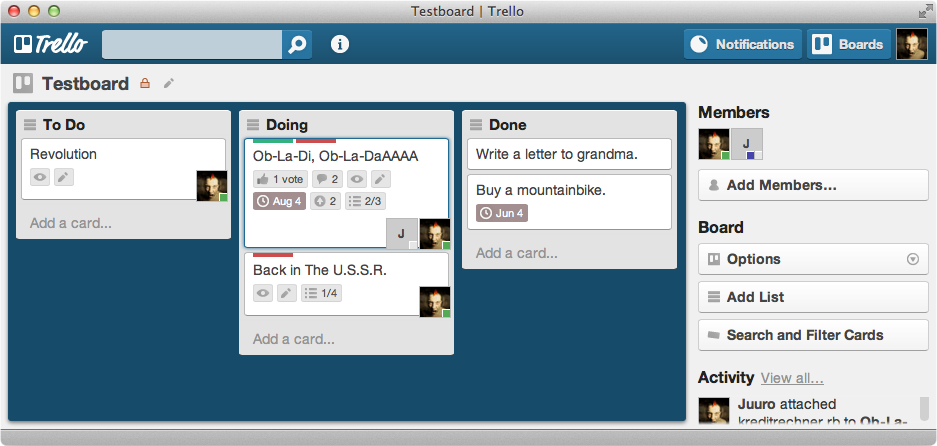
\includegraphics[width=\textwidth]{figures/trello}
\caption{A Trello board.}
\label{fig:trello}
\end{figure}

There is the concept of the so called \emph{boards} which contain several configurable lists. Figure \ref{fig:trello} shows a board with the three standard lists \emph{To Do}, \emph{Doing} and \emph{Done}. In these lists the user can create to-do items. These to-do items are called \emph{cards}. The cards can contain several additional data. Each card has a title and maybe a description, some assigned members, a due date, some labels, votes, checklists, comments and attachments. The creator of the board is the owner in the first place and the owner can add other Trello users to his boards and cards. So everone who's working on a project can see whats going on at the moment. Users who are assigned to a board can even create new to-do items by themselves. If somebody works at more than one company with many projects each there is the concept of \emph{organizations}. This is useful in order to ensure a clear separation.

\begin{figure}[htb]
\centering
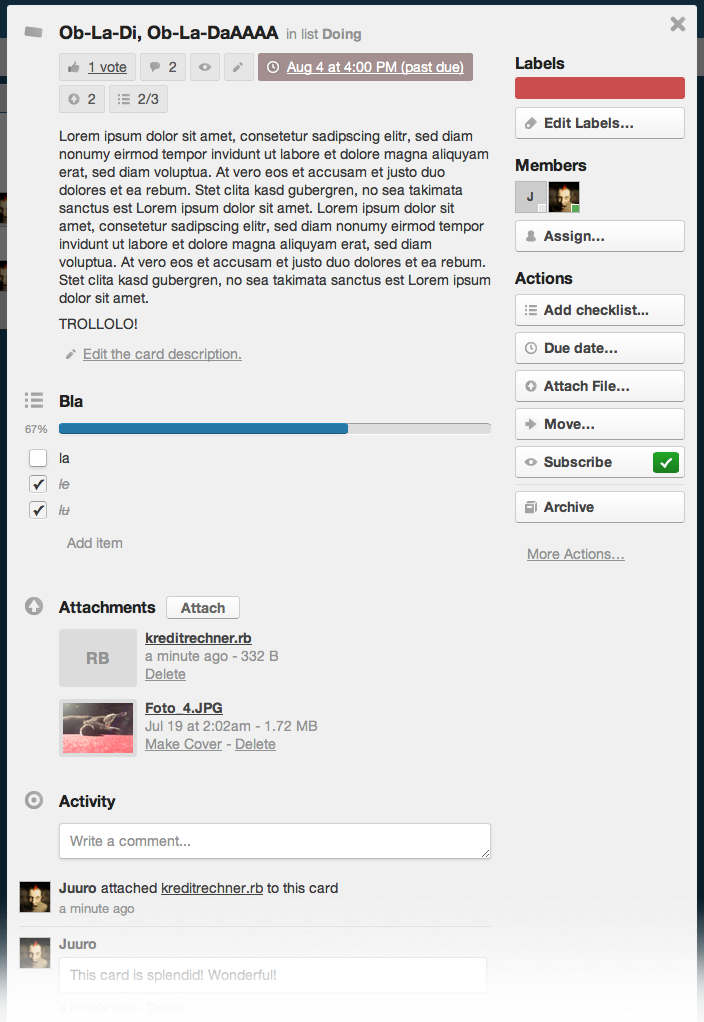
\includegraphics[width=\textwidth]{figures/trello-card}
\caption{A opened card in Trello.}
\label{fig:trello-card}
\end{figure}

\subsection{Why Trello}\index{Trello}
Trello is not just one of hundreds of thousands of to-do applications. It is streamlined for the purposes of small businesses. So it is perfect for the needs of a university with small groups of people working on the same things. Trello has already prooved its value for several months. The Trello website is written in HTML 5\index{HTML!5} with the use of AJAX\index{AJAX} where it makes sense. Trello provides an iOS\index{iOS} \cite{trello:ios} and Android\index{Android} \cite{trello:android} app. Both are constantly evolving. So the system is state-of-the-art. In addition the company behind Trello is not just a start-up with three employees, which is also of importance. A product of a small business, which is just based on the enthusiasm of the founders often doesn't last long. Fog Creek Software is over ten years old and has several products.

The first aim was to see the due dates of the cards someone is assigned to in Google Calendar. But thinking about that there were many other use cases for small scripts which could run as cron jobs on a server to serve several regular tasks. These scripts are described in more detail in Chapter 3.

\subsection{Trello API}\index{API}
Trello has an API \nomenclature{API}{Application Programming Interface} which is still in beta. But it is already very extensive. \cite{trello:docu}

\subsubsection{Authentification}
The access the private boards in Trello\index{Trello} there has to be some kind of authentication. For user applications with a frontend the Trello API provides OAuth2. But because of the concept of OAuth2 the user is required to enter his Trello username and password. \cite{oauth} My scripts are supposed to run on servers as cron jobs. There is no user who could manually enter data. For this kind of applications Trello provides a key/token-system. Every user has a private key. With this key the user can generate a token. This token will be sent along every request to the Trello API. The token tells Trello which scope the request can see. While generating a token the user can specify the scope of the token and when it will expire. The possible expriation date of a token is between one day and never. In our case we will use \emph{never}. To generate a token one has to visit a special URL:
\texttt{
https://trello.com/1/authorize?key=SUBSTITUTEWITHYOURPRIVATEKEY \&name=My+Application\&expiration=never\&response\_type=token \&scope=read,write}
In this example the token would never expire and could read and write everything the user can access with the API. Other valid values instead of \texttt{never} for expiration would be \texttt{1day}, \texttt{30days}. \texttt{30days} is the default value. \cite{trello:gettingstarted}

\subsubsection{REST}\nomenclature{REST}{Representational State Transfer}
The Trello API is a \emph{RESTful} web API. That means that the API is conform to the REST design model. REST is a common style of software architecture for distributed systems. It's built on four of the HTTP request methods: GET, POST, PUT and DELETE. An implementation of a REST web service follows four basic design principles:
\begin{itemize}
	\item Use HTTP\nomenclature{HTTP}{Hyper Text Transfer Protocol} methods explicitly.
	\item Be stateless.
	\item Expose directory structure-like URIs\nomenclature{URI}{Uniform Resource Identifier}.
	\item Transfer XML\nomenclature{XML}{Extensible Markup Language} , JSON\nomenclature{JSON}{JavaScript Object Notation}, or both.
\end{itemize}
\cite{rest}

Following these conventions a GET URL of a RESTful web service looks like this:
\begin{center}
\texttt{https://api.trello.com/1/cards/4fc8dd3e1b9ecf0c3571902f? key='PRIVATEKEY\&token=TOKEN}
\end{center}
This is a GET request to get a specific card with the id \texttt{4fc8dd3e1b9ecf0c3571902f}. If this URL\nomenclature{URL}{Uniform Resource Locator} is visited in a browser (with correct \emph{key} and \emph{token}) the browser will show plain JSON. In order for Ruby to be able to work with it, it must somehow capture this data. To fulfill the requirements of REST in Ruby there are several gems. Here the RestClient gem is used. This GET request with the RestClient gem in Ruby looks like \ref{listing019}.

\begin{lstlisting}[aboveskip=1\baselineskip, caption=GET request using RestClient., label=listing019]
member = RestClient.get('https://api.trello.com/1/cards/4fc8dd3e1b9ecf0c3571902f?key='+$key+'&token='+$token)
pp JSON.parse(member)
\end{lstlisting}

In comparison to the open-uri library, which is included in the Ruby standard library, it's much more tidied up when it comes to POST requests.

\begin{lstlisting}[aboveskip=1\baselineskip, caption=POST request using RestClient., label=listing009]
response = RestClient.post(
	'https://api.trello.com/1/boards',
	:name => board['name'], 
	:desc => board['desc'],
	:key => $key,
	:token => $token
)
\end{lstlisting}

\begin{lstlisting}[aboveskip=1\baselineskip, caption=POST request with open-uri., label=listing010]
uri = URI('https://api.trello.com/1/boards')
req = Net::HTTP::Post.new(uri.path)

req.set_form_data(
	'name' => board['name'], 
	'desc' => board['desc'],
	'key'=>$key,
	'token'=>$token
)

Net::HTTP.start(uri.host, uri.port, :use_ssl => uri.scheme == 'https') do |http|
	response = http.request(req)
end
\end{lstlisting}

Listing \ref{listing009} and listing \ref{listing010} show the very same API call. But \ref{listing009} is realised with RestClient and listing \ref{listing010} with open-uri. Not only is the open-uri code much longer, but open-uri also doesn't detect the correct scheme from the given URI. If the call should performed in HTTPS this has to be set explicitly. This implies that for the handling of RESTful web services RestClient is the better choice.


\section{Ruby}\index{Ruby}
Ruby is a modern general-purpose object-oriented programming language. Its big difference to most other languages is that it focuses on humans rather than computers. 

Yukihiro Matsumoto, the designer of Ruby, once said:
\begin{quote}
Ruby is simple in appearance, but is very
complex inside, just like our human body.\cite{ruby:talk}
\end{quote}

That means that Ruby\index{Ruby} is very easy to read and is intuitive for humans even though it can perform complex tasks. This is achieved with English keywords instead of brackets and curly brackets. The result for the programmer of this consistent philosophy is a very easy to read language which is also very plain. Because of the English words instead of abstract characters Ruby is easy to understand. Even non-programmers are mostly able to understand whats going on. So programmers produce a lot fewer errors while writing the code. A wrongly spelt word is more intuitively recognisable than a missing bracket or semicolon. \cite{ruby:about} More about Ruby can be found at \url{http://www.ruby-lang.org}.

\subsection{RubyGems}\index{RubyGems}
Ruby has many methods and classes every Ruby installation provides\footnote{Libraries that are included with the Ruby standard library: \url{http://www.ruby-doc.org/stdlib-1.9.3/}}. But there are hundreds of extensions for special use cases – to communicate with RESTful Web APIs for example – made by third party developers. In Ruby such extensions are called \emph{gems}. To manage and publish these third party libraries there is the standard \emph{RubyGems}. It provides a standard format for third party libraries for Ruby, a tool to manage the installation of gems and a server for distributing the gems. \cite{ruby:gemdev} Some Ruby distributions are delivered with several gems. Gems can be added to an existing Ruby installation at any time. 

To install an additional gem on a Unix operating system the following command can be used:  
\begin{center}
\texttt{gem install gemname}
\end{center}
Where \texttt{gemname} is the name of the respective gem. If the installation performed without errors, the gem is ready to use. \cite{ruby:gemdoc}

To use an installed gem in a Ruby\index{Ruby} script the following code at the top of the script before the code starts is necessary:

\begin{lstlisting}[aboveskip=1\baselineskip, caption=Using the gem \emph{gemname}, label=listing001]
require 'gemname'
\end{lstlisting}
Again, \emph{gemname} stands for the name of the respective gem. If any gems that are not part of the Ruby standard library are used in this script, they are listed at the beginning of the related description. Further information at \url{http://doc.rubygems.org} and \url{http://rubyforge.org/projects/rubygems/}. Additionally \url{http://rubygems.org} is a reference book like website for Ruby gems.

\subsection{Ruby and MySQL}\label{rubymysql}
In order to access databases in Ruby there are additional libraries needed. The Ruby standard library doesn't support any databases. To enable support for databases in Ruby additional libraries are needed. In this API wrapper the MySQL gem is used. This gem is an API wrapper around the MySQL C client API.\todo{true?} MySQL is used here because it is the most popular open source database. \cite{mysql:popularity} It is especially popular for the use in web applications. The scripts described here access primarily web applications, so it's the right choice to support MySQL.

\begin{lstlisting}[aboveskip=1\baselineskip, caption=Initialising database connection., label=listing033]
my = Mysql.init
my.options(Mysql::SET_CHARSET_NAME, 'utf8')
my.real_connect(dbhost, dbuser, dbpassword, db)
my.query("SET NAMES utf8") (*@ \label{line029} @*)	
\end{lstlisting}

Listing \ref{listing033} above shows the initialisation of a new connection to a MySQL database with the Ruby MySQL gem. The variable \lstinline{my} is a new database handler. If the correct charset isn't set it won't work. The host, the user, the password and the database name should be stored in seperate variables so they are easily editable. \lstinline{SET NAMES utf8} in line \ref{line029} of listing \ref{listing033} is a first execution of a MySQL query. It tells the server the charset name of future connections. In this example the server expects all future queries as UTF8 \nomenclature{UTF-8}{8-Bit UCS Transformation Format}\nomenclature{UCS}{Universal Character Set} charset.

MySQL statements can executed directly or as \emph{prepared statements}. The example in line \label{line029} of  \ref{listing033} is a normal statement which is executed directly. Listing \ref{listing034} shows a longer example. 

\begin{lstlisting}[aboveskip=1\baselineskip, caption=Example for a directly executed MySQL query., label=listing034]
response = my.query(" 
	SELECT fieldname1 (*@ \label{line0305} @*)
	FROM tablename 
	WHERE  fieldname2=value
	AND fieldname3=value (*@ \label{line031} @*)
")
response.each do |row|
	puts row (*@ \label{line032} @*)
end
\end{lstlisting}

The MySQL statement between line \ref{line0305} and \ref{line031} responses with data. So the result of the query must be read somehow. The response of a \lstinline{SELECT} statement is an array of rows from the given table. So to get the lines of the response table the \lstinline{each} method is used to iterate through the array and print each row.

\begin{lstlisting}[aboveskip=1\baselineskip, caption=\texttt{joomlaMultiple.rb} usage., label=listing029]
statement = my.prepare("
	INSERT INTO tablename (
		fieldname1,
		fieldname2
	) 
	VALUES (
		?,
		?
	)
")
statement.execute value1, value2 (*@ \label{line033} @*)
statement.execute othervalue1, othervalue2 (*@ \label{line034} @*)
\end{lstlisting}

The listing above shows how the MySQL library for Ruby handles prepared statements. The big difference to directly executed statements are the wildcards in the \lstinline{VALUES} part. It's more like a template for a statement. Although the statement doesn't contain all required values it's sent to the underlying DBMS\nomenclature{DBMS}{Database Management System} of MySQL. The DBMS is able to perform query optimisation on this statement template. To fill in the actual values the statement must be executed with the \lstinline{execute} method. The lines \ref{line033} and \ref{line034} are two executions of the specified statement. In this step the wildcards are replaced by the wildcards. The DBMS performs additional query optimising if needed. Sometimes query optimisation depends on the values of the fields. Prepared statements can be executed multiple times. That saves performance, because the initial query optimisation must be performed only once. In addition performed statements are safer that directly executed statements. Because the DBMS processes the MySQL code seperately to the actual data it can distinguish between valid and invalid data. The DBMS checks every given value before writing it to the database. Because of that SQL injection isn't possible with prepared statements. So for every MySQL statement that writes data to the database it's reasonable to use prepared statements. \cite{mysql:rubydoc}


\section{JSON}\index{JSON}\label{jsonsec}
All the responses to Trello\index{Trello} API\index{API} calls use JSON\footnote{RFC\nomenclature{RFC}{Request For Comments} document for JSON: The application/json Media Type for JavaScript Object Notation (JSON)  \url{http://www.ietf.org/rfc/rfc4627.txt}}. It is a subset of the JavaScript programming language. Despite its relation to JavaScript it's language independent. JSON is a data-interchange format like XML. But JSON is built on two structures. One is a list of key/value pairs. In most programming languages this is realised as a hash, struct, object or associative array. The other structure is an ordered list of values. This is realised as an array, list, vector or sequence in popular programming languages. In JSON itself these structures are called \emph{object} and \emph{array}. Objects start and end with curly brackets. Each key is followed by a colon and the key/value pairs are separated by commas. Arrays start and end with squared brackets. The values are separated by commas. Both can be arbitrary nested. Everytime one of the scripts saves content to any other place than Trello it's in the JSON\index{JSON} format, too. That's because it guarantees easy compatibility with Trello. JSON\index{JSON} can also be saved in files. A JSON\index{JSON} file has the suffix \texttt{.json}. \cite{json}

\begin{lstlisting}[aboveskip=1\baselineskip, caption=JSON example., label=listing0075]
{
    "id": "4eea4ffc91e31d1746000046",
    "name": "Example Board",
    "desc": "This board is used in the API examples",
    "lists": [{
        "id": "4eea4ffc91e31d174600004a",
        "name": "To Do Soon"
    }, {
        "id": "4eea4ffc91e31d174600004b",
        "name": "Doing"
    }, {
        "id": "4eea4ffc91e31d174600004c",
        "name": "Done"
    }]
}
\end{lstlisting}

In listing \ref{listing0075} a JSON example is shown. This is the response of

\begin{center}
\texttt{https://api.trello.com/1/boards/4eea4ffc91e31d1746000046? lists=open\&list\_fields=name,desc\&key=PRIVATEKEY\&token=TOKEN}
\end{center}

The JSON in listing \ref{listing0075} starts with a curly bracket. That means the uppermost structure is an object. Here are a few key/value pairs like \texttt{"id": "4eea4ffc91e31d1746000046"}. The key \texttt{"list"} has an array as value. So their value is in squared brackets. Each element of the array is an object again.

To process the received JSON Ruby needs to parse it first. For that purpose there is the a gem simply called \emph{JSON}. It parses the JSON with the 

\begin{center}
\lstinline{JSON.parse(receivedJson)} 
\end{center}
command, where \lstinline{receivedJson} is a variable that contains the plain JSON received from the Trello API with a GET request. After the parsing the JSOn objects are now represented as Ruby Hashes and the JSON arrays as Ruby arrays. To post content to the Trello API it has to be in JSON, too. So there is another method of the JSON class in Ruby which generates JSON from Ruby hashes and arrays. 

\begin{center}
\lstinline{JSON.generate(hashBoards)} 
\end{center}

The result is a valid JSON formatted string, ready to write to a JSON file or to send to an API.